%
% Modified by Sameer Vijay
% Last Change: Wed Jul 27 2005 13:00 CEST
%
%%%%%%%%%%%%%%%%%%%%%%%%%%%%%%%%%%%%%%%%%%%%%%%%%%%%%%%%%%%%%%%%%%%%%%%%
%
% Sample Notre Dame Thesis/Dissertation
% Using Donald Peterson's ndthesis classfile
%
% Written by Jeff Squyres and Don Peterson
%
% Provided by the Information Technology Committee of
%   the Graduate Student Union
%   http://www.gsu.nd.edu/
%
% Nothing in this document is serious except the format.  :-)
%
% If you have any suggestions, comments, questions, please send e-mail
% to: ndthesis@gsu.nd.edu
%
%%%%%%%%%%%%%%%%%%%%%%%%%%%%%%%%%%%%%%%%%%%%%%%%%%%%%%%%%%%%%%%%%%%%%%%%

%
% Chapter 3
%

\chapter{TWO PROTON TRANSFER AT NOTRE DAME}
\label{chap:2pExpt}

\begin{comment}
Give an overview of the requirements for two-proton transfer and say that ND has a buncher and a Tandem accelerator that goes up to 10 MV so we can get beam energies up to 30 MeV for \He{3} and we have a beamline with a long flight path SO we can do this experiment.
\end{comment}

The previous chapter demonstrated the interest in studying \reaction ; this chapter will discuss the beam production and experimental setup.  The most important peices of the setup are the beam energy, the beam bunching, and the optimization of the neutron detector to provide excellent timing information.   

% detecting neutrons
% this means we need timing information
% so the beam must be bunched
% and the detector must be built to give good timing
% and placed to give good timing
Measuring the time of flight (TOF) of the neutron to sufficient accuracy requires both beam bunching and a long neutron flight path.  In a continuous beam, there is no way to know which \He{3} was associated with a neutron event in the detector, and therefore no way to determine TOF.  Bunching the beam so that clumps of \He{3} arrive at the same time and providing a signal correlated to their arrival at the target allows a TOF measurement with a precision determined by the time-width of the bunch.  This limit on time resolution constrains the distance between the target and detector.  

% interested in 0+ distribution
% and there's an ideal beam energy for that
% and that constrains the distance between the target and neutron detector
As discussed in the previous chapter, the purpose of this experiment is to understand the distribution of the \zp state.  The maximum \zp cross-section for \reaction requires a beam energy near 18 MeV, but the resolution of the neutron detector decreases with increasing neutron energy.  The beam energy must be as close to 18 MeV as possible while still providing sufficient resolution.

States populated through different $l$ transfer can be discriminated by their angular distributions.  The DWBA calculations in the previous chapter show the expected maximum and minimum of the \zp cross-section to be at 0 and 22 degrees, respectively. 


\section{Beam Production at Notre Dame}
The beam delivered to the target is 16 MeV bunched \He{3}.  In this section, we will follow the beam through its production and acceleration.

The Helium Ion Source (HIS) provides negative \He{3} ions to the accelerator.  A duoplasmatron ion source filled with \He{3} gas uses a discharge across high voltage to convert some of the gas into plasma.  Electrostatic elements extract positive \He{3} ions from the plasma and accelerate them into a canal filled with lithium vapor.  Lithium is crucial to creating negatively charged beam because it donates electrons generously, and a small fraction of the \He{3} becomes negatively ionized after passing through the canal.  A dipole magnet after the ion source removes the carbon, oxygen, and other impurities that contaminate the \He{3} beam.  Movable, thick tungsten slits block much of the beam, allowing only beam within a small range of magnetic rigidity to pass through to the accelerator.

The accelerator at Notre Dame is a tandem Van deGraaff accelerator made by High Voltage Engineering Corporation.  Its maximum terminal potential is 10 MV.  Negatively charged beam enters and accelerates toward the positive terminal, located in the center of the machine. A thin carbon foil ($\sim$ 3 $\mu$g/cm$^2$) in the center of the machine strips electrons from the beam.  The now-positive beam accelerates again, away from the positive terminal. In general, the final energy of a particular beam with is 

\begin{equation}
E = E_{HIS} + (1+q)eV_T
\end{equation}

where $V_T$ is the terminal voltage, $E_{HIS}$ is the energy of the beam exiting the HIS, and $q$ is the charge state of the beam after passing through the carbon foil.  \He{3} beam is fully stripped of its electrons by the carbon foil, and so the terminal voltage required to produce 16 MeV \He{3} is 5.33 MV, a comfortable operating voltage for the accelerator.  Keeping this terminal voltage stable isthe difficult thing.  

Dipole magnets with a magentic field strength $B$ will bend a particle with momentum $p$ and charge $qe$ in a circle of radius $R$.  The product of the field strength and the radius of the path, $BR$, is of interest in beam physics because the radius of the path is essentially fixed by the position of the beamline and is called the rigidity.

\begin{equation}
BR = \frac{p}{qe} = \frac{\sqrt{2mE}}{qe}
\label{eqn:rigidity}
\end{equation}

Since the mass and charge of the desired beam are fixed, selecting beam at a fixed radius exiting a dipole defines its energy.  A large dipole magnet at the exit of the tandem can work in a feed-back circuit to regulate the terminal voltage.  Two horizontal slits at the dipole exit are only several milimeters apart and define a narrow range for the radius traveled by the beam.  If the terminal voltage drifts off its set point, the trajectory of the majority of the beam will travel a larger radius and hit the slit.  This slit current feeds back into the accelerator electronics, causing a decrease in terminal voltage that returns the beam energy to the pre-selected value.  Such regulation is limited by the stability of the magnetic field of the dipole.  This analyzing magnet is calibrated against the nuclear magenetic resonance (NMR) of hydrogen and using it to regulate the teriminal voltage reduces the ripple in the voltage to 10 kV.


\subsection{Beam Focusing and Selection}

Immediately after acceleration and energy selection, the beam is narrowly defined.  However, the beam must travel ?? m  to the target.  Many focusing and steering elements along the way are necessary to obtain a reasonable transmission rate and ensure that the beam is well-focused at the target.  Two Einzel lenses [need cite] focus the beam before it enters the accelerator, and a set of electrostatic steerers before and after the accelerator are enough to position the beam before it enters the energy-selecting dipole magnet.  Quadrupole doublet magnets focus the beam as it travels through the target rooms, and another set of steerers allows correction of the beam position and angle.  The final focusing element before the target are two large-bore, variable-strength solenoid magnets [cite needed] that focus the beam to a spot approximately 2 mm in diameter.

% figure: beamline
\begin{figure}[htp]
\centering
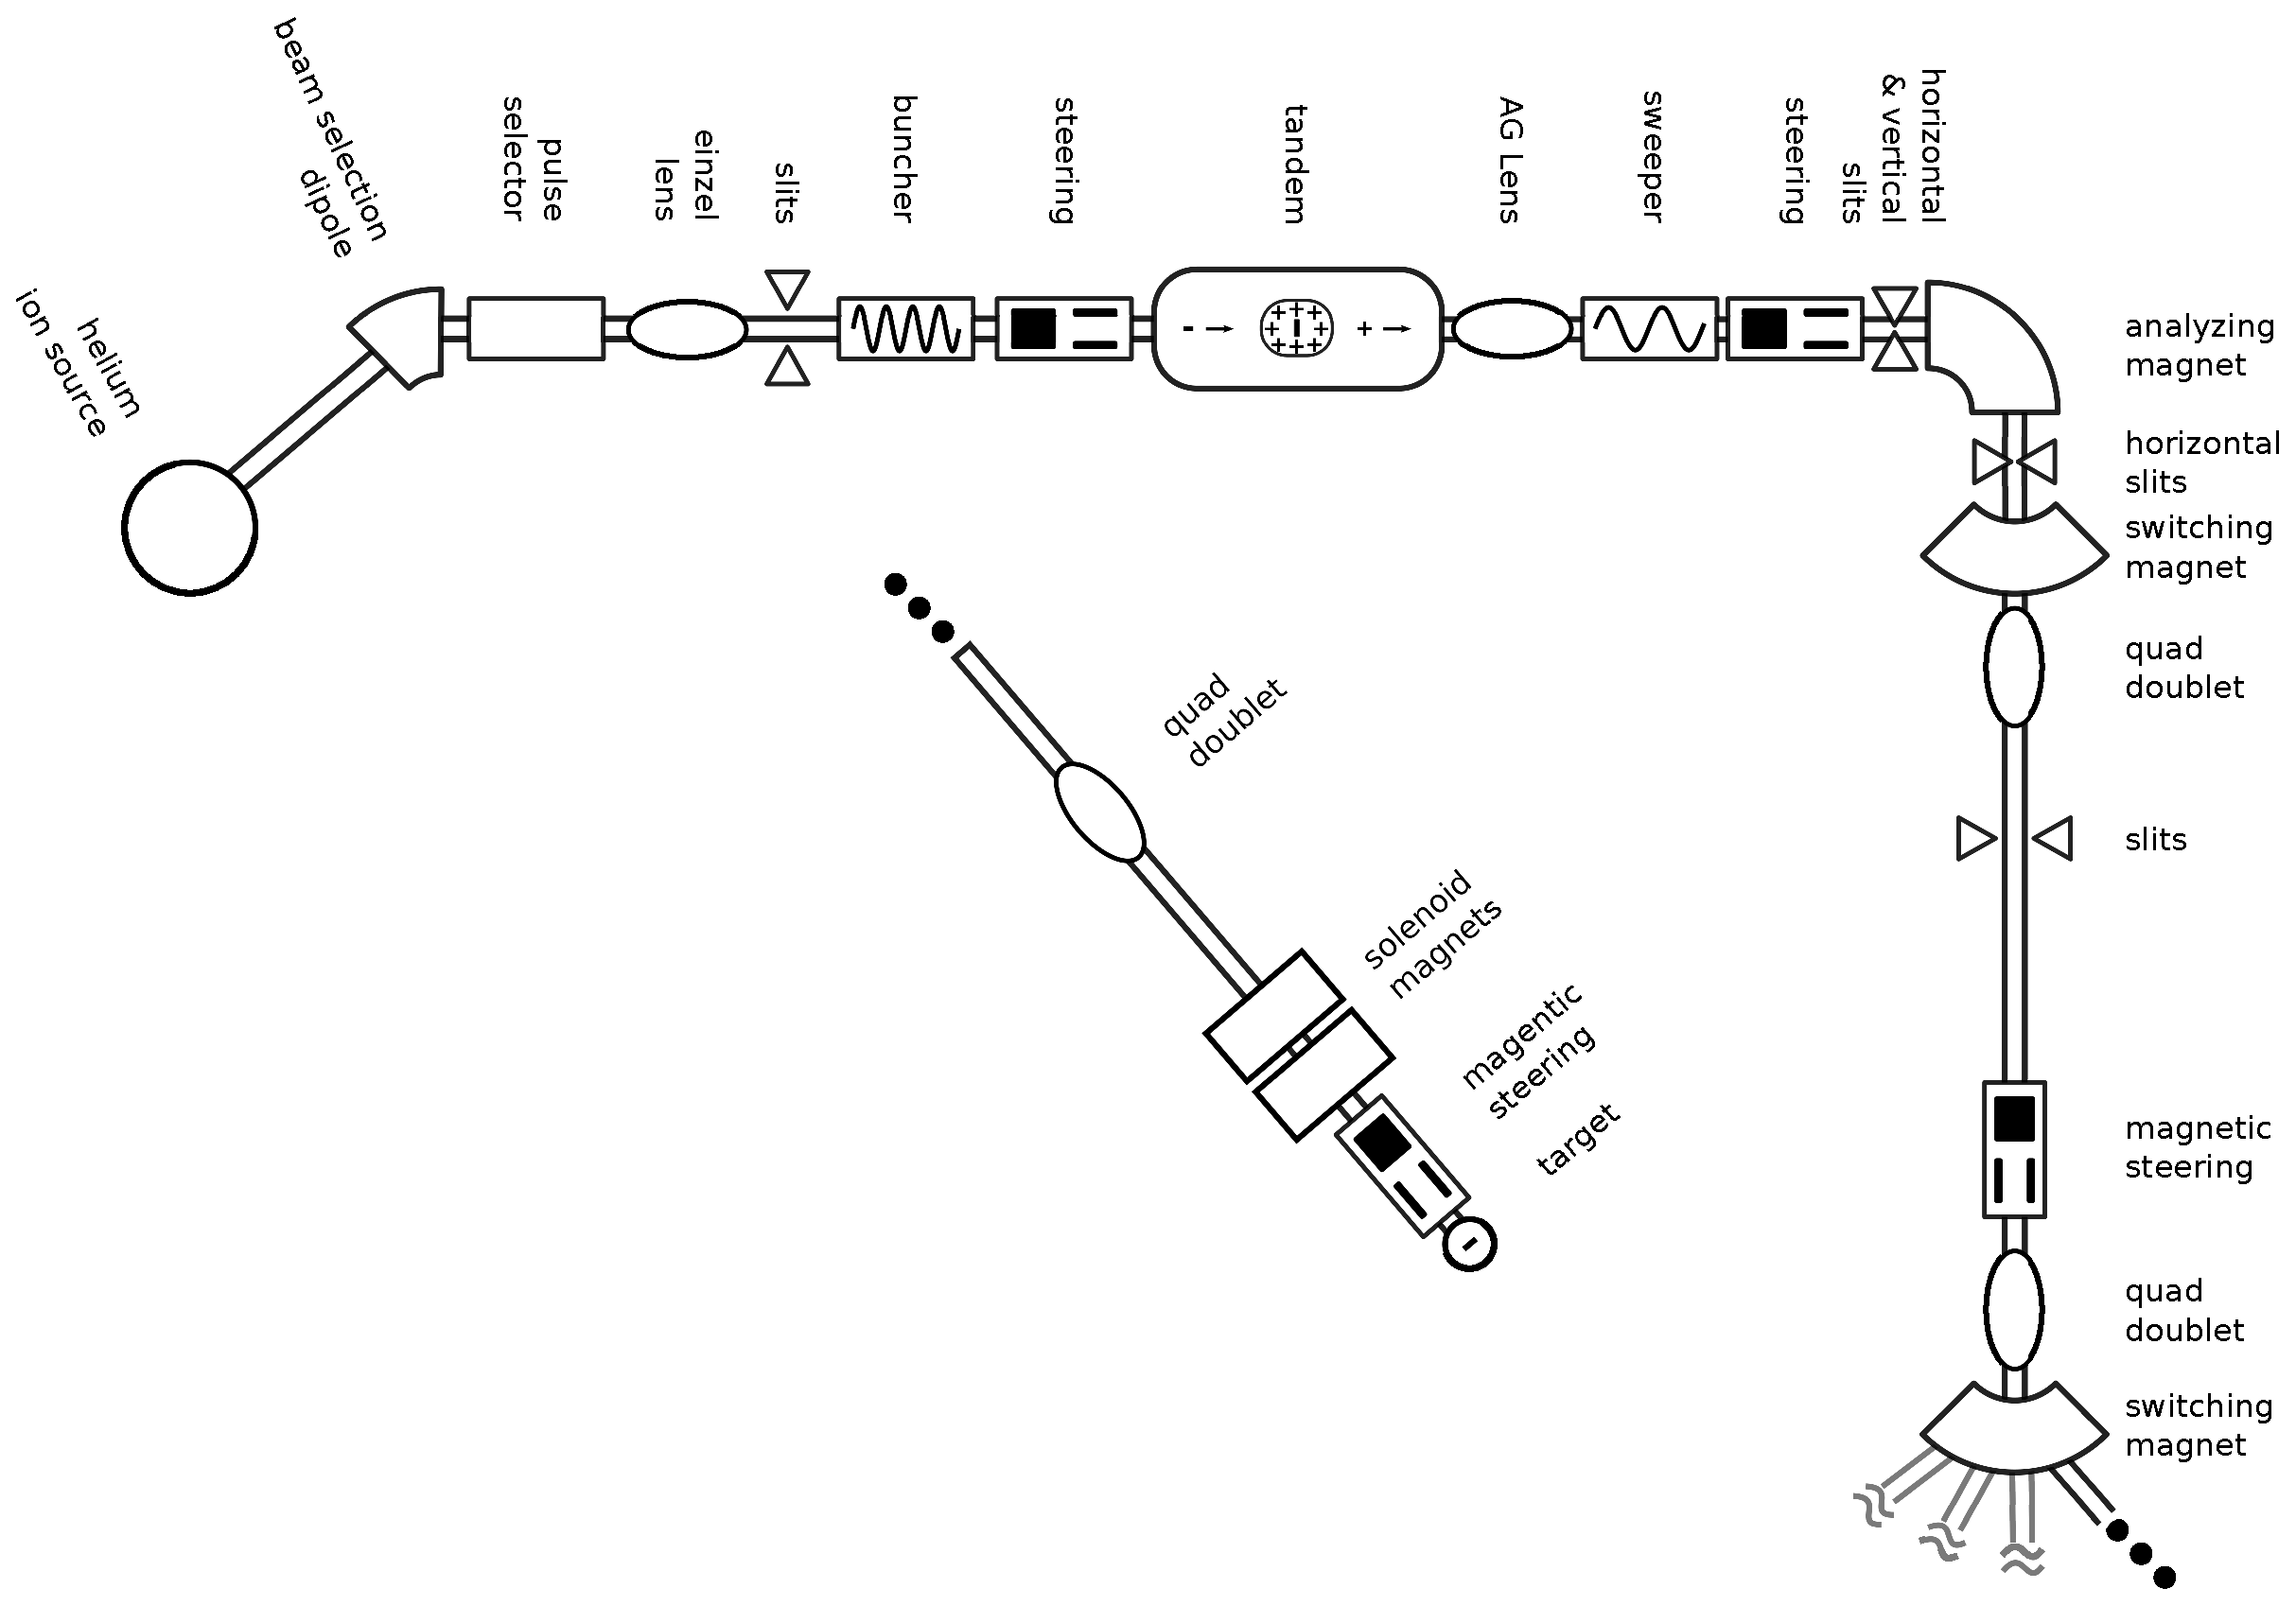
\includegraphics[width=1.0\textwidth]{figures/NSL_beamline.eps}
\label{fig:beamline}
\caption{Beam production at Notre Dame.}
\end{figure}

\subsection{Beam Bunching}

Continuous beam would make it impossible for our detectors to determine the neutron TOF.  It is possible to bunch the beam so that ``bunches'' of \He{3} arrive at the target, each bunch having a time spread of approximately one ns. There are three components to the bunching system at Notre Dame.  The first is the buncher itself, which pushes about 40\% of the beam into discrete bunches.  The remaining 60\% is a continuous background and must be removed with the 'sweeper'.  Together, the buncher and sweeper provide bunches of beam that are 1 ns wide at the target and separated by 101 ns, with no beam in between.  With the detector 15 m away from the target, some of the slow neutrons coming from the reaction have a TOF in excess of 300 ns.  A pulse-selector is used to eliminate three out of every four bunches to avoid overlapping energetic neutrons from the current beam bunch with slow neutrons from the previous bunch.  The buncher, sweeper, and pulse-selector together provide clean bunches of beam separated by 400 ns.  The rest of this section describes how each of these components works.

The beam buncher at Notre Dame works by slowing down particles that would arrive too early at the target and speeding up particles that would be arriving too late.  To achieve this, two grids perpendicular to the beam connect to a radiofrequency (RF) power supply to create a time-varying electric field.  If the electric field were a sawtooth wave in time, the beam bunches would contain all the beam \cite{LynchBunching}.  As illustrated in \ref{fig:bunching}, decelerates the early portion of the beam and accelerates the late portion of the beam.  The strength of the field determines the distance at which the bunch will be narrowest, with a stronger field bringing the bunch into focus earlier than a weaker field.  The pure sawtooth field is able to bunch 100\% of the incoming beam because it immediately resets after its linear portion.  Commercially available RF power supplies, however, generally vary sinusoidally in time.  At Notre Dame, a single frequency buncher that operates at 9.85 MHz is used.  While the RF signal is increasing approximately linearly with time, beam is bunched exactly as if the field were a pure sawtooth wave.  When the electric field approaces a maxiumum or minimum, little bunching occurs, and when the electric field is decreasing, de-bunching occurs.  The sinusoidal RF supply results in nanosecond (ns) wide bunches contain $\sim$40\% of the beam arriving at the target every 101 ns superimposed on a continuous background of the remaining beam.  This continuous beam would render our time signal useless and must somehow be removed.

% figure: how a beam buncher works
\begin{figure}[htp]
\centering
\includegraphics[width=1.0\textwidth]{figures/beamBunching.eps}
\label{fig:bunching}
\caption{Beam bunching using a time-varying electric field.  Each dot represents a beam particle, and the vertical gray bars represent the bunching electrodes.  To bunch one section of beam, particles arriving first must be slowed down, while particles arriving last must be sped up.  A linearly increasing field does exactly this.  If the wave is a perfect sawtooth, there is no time during which beam is not being bunched - that is, all the beam is bunched.  Notice also that beam does not exit the buncher in a tight bunch; as time passes, beam drifts together.  The time until the bunch is at its narrowest depends on the amplitude of the electric field applied by the buncher.}
\end{figure}

The ``sweeper'' provides a sinusoidal electric field that is timed to deflect the continuous beam between the bunches.  A set of vertical slits immediately after the sweeper removes the deflected beam.  Variable delays allow adjustment of the timing between the buncher and the sweeper and must be optimized for a particular beam.  Even a few-nanosecond change in the timing can affect which portion of the beam is swept away. 

%figure of beam profile and sweeper

It is possible to take data without pulse selection, but because the spread in TOF of the neutron spectrum is in excess of 300 ns, it complicates the TOF spectrum considerably.  With bunches arriving at the target every 101 ns, it will be impossible to tell if a neutron is very fast and associated with the current bunch or very slow and associated with the previous bunch.  The resulting spectrum is shown in Figure \ref{fig:PSvsNPS_TOF}.

% figure: the considerably complicated spectrum
\begin{figure}[htp]
\centering
\subfloat[][]{
   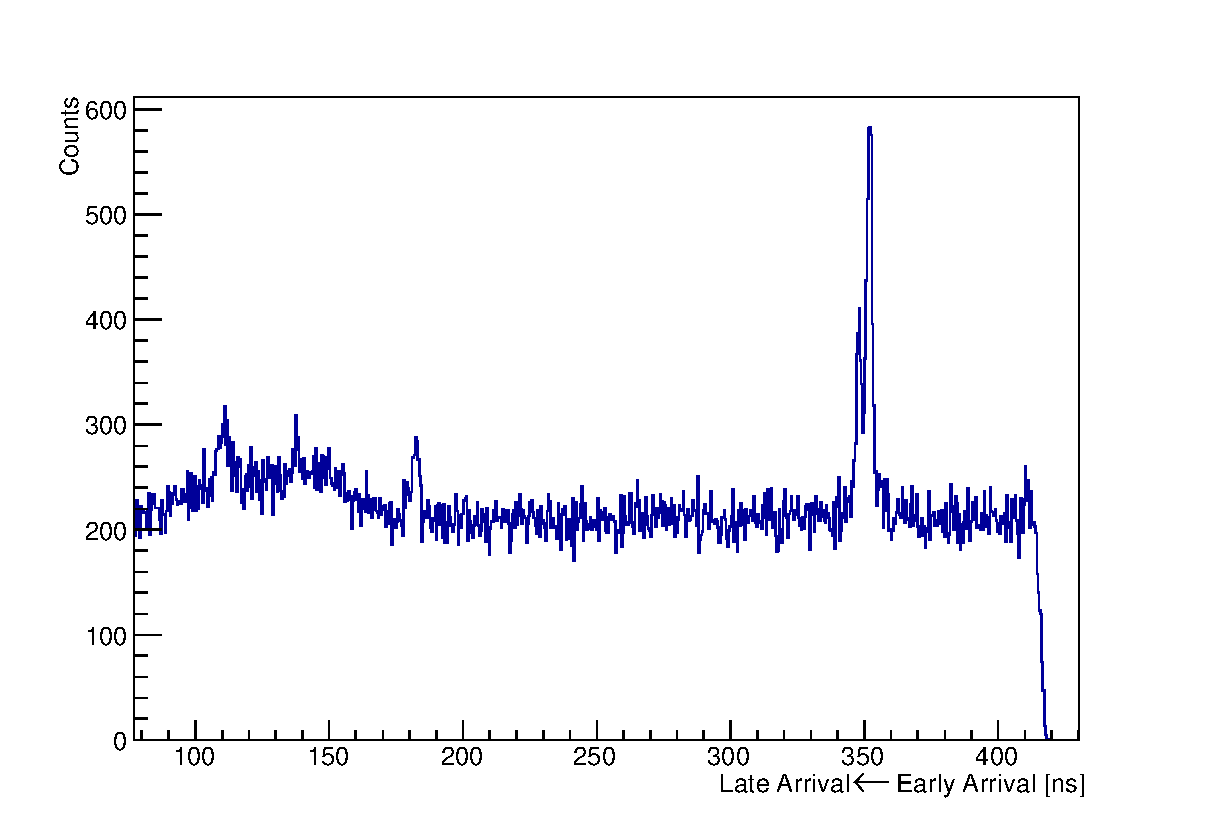
\includegraphics[width=0.4\textwidth]{figures/PS_BarA_Sep.eps}	
}
\subfloat[][]{
	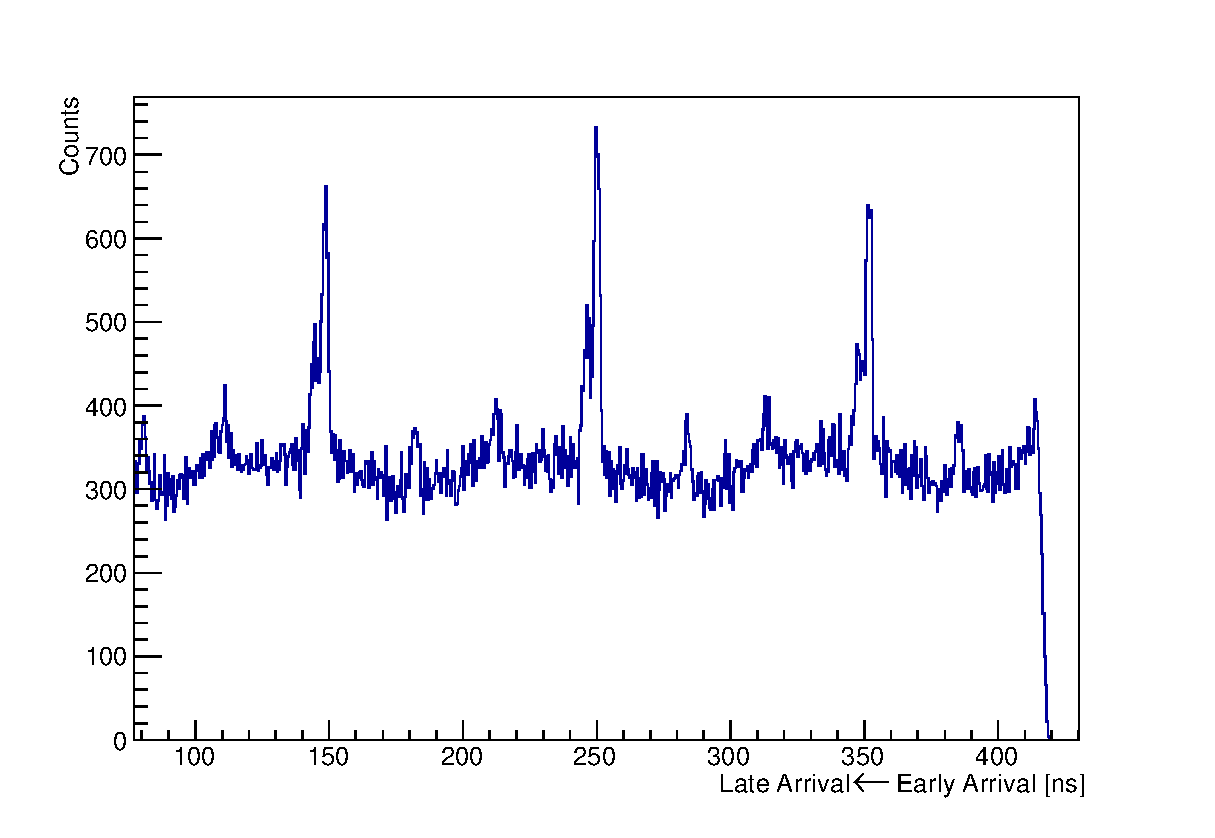
\includegraphics[width=0.4\textwidth]{figures/NPS_BarA.eps}
}
\label{fig:PSvsNPS_TOF}
\caption{Figure A shows timing spectrum from a pulse-selected beam.  The timing spectrum in figure B is from beam with no pulse selection.  Both timing spectra are from a \He{3} beam on a \Ge{76} target.}
\end{figure}

To give all the neutrons resulting from one beam bunch time to reach the detector before the next bunch strikes, a ``pulse selector'' eliminates three of every four bunches, resulting in 404 ns between each bunch at the cost of beam intensity.  The pulse selector is located before the accelerator and consists of two parallel plates, one held at ground and the other at +400 V.  A fast switch (SCR) connects the high-voltage plate to ground, letting the selected bunch through without deflection.  Vertical slits immediately after the pulse selector remove deflected beam, while undeflected beam passes through to the accelerator.  While the beam width is only one ns at the target, at the sweeper the bunch is approximately 80 ns wide, so the SCR must hold the plate at ground for 80 ns to let the entire bunch through.

% figure: slow neutrons and their dissappearance

Beam bunching and pulse selection reduce available beam current - the swept beam current is only 40\% $\times$ $\frac{1}{4} = 10$\% of the non-bunched current.  But without bunched beam it would not be possible to distinguish the neutrons of interest in the (\He{3},n) transfer reaction.  Increased beam current would improve statistics on \reaction, but the HIS was already operating at its full output for these experiments.

\section{The Target Chamber}
\begin{comment}
target
thin stainless stell wall
Si detector
BaF2 detector
\end{comment}

The 16 MeV \He{3} beam has been bunched, swept, pulse-selected, and steered and focused onto the target.  The bunches that were 80 ns wide before the accelerator have converged into 1 ns wide bunches at the target.  The target is at the center of a thin-walled stainless steel chamber that has a small gold-lined faraday cup.   

To measure the absolute scale of the cross-section, it is necessary to know the number of particles incident on the target.  This is done in several ways.  A Si detector placed inside the target chambermonitors \He{3} scattered off the targets.  Another measure of the beam current is the charge measured from the faraday cup.  Additionally, a BaF2 detector located just outside the chamber counts $\gamma$ radiation produced by beam interactions in the target.  

% figure: the target chamber & its detectors

\section{The Neutron Detector}
\begin{comment}
Discuss neutron wall briefly.  Can reference NIMA paper. Explain why it's important that it's wide-angle. 
\end{comment}

The resulting products of a two-proton transfer onto \GeTargets are a neutron and a \SeProducts nucleus.  Measuring the outgoing neutron is possible becuase the neutron, lacking charge, is not likely to interact with remaining material in the target or even the stainless steel target chamber.  For the detectors themselves to observe the neutrons, the detector must provide protons with which the neutrons can strongly interact with.  Unlike charge particle detection, neutrons rarely deposit their full energy in a detector.  Neutrons can only deposit all their energy when the collide head-on with a proton.  Much more likely is a glancing interaction, where the neutron imparts only some of its energy to the proton.  The measured energy spectrum of monoenergetic neutrons ranges from the detector threshold up to the neutron's full energy, making it impossible to determine the energy of the neutron from its deposited energy.  Instead, the time of flight (TOF) between the target and the detector is used to distinguish neutrons of differing energies.  The neutron detector is optimized to provide precise timing information.       
% figure of charged-particle energy spectrum
% figure of neutron energy spectrum

The neutron detector [cite neutwall] consists of 16 large (1.5 m $\times$ 0.15 m $\times$ 0.05 m) bars of commercially available scintillator with excellent timing response [reference BC408].  Each plastic scintillator bar is equipped with two fast-risetime photomultiplier tubes (PMT's) at opposite ends.  The signal risetimes are approximately 5 ns and by processing the signal with constant fraction discriminators (CFD's), the timing resolution of the PMT's is sub-nanosecond.  Additionally, PMT's on opposite ends of the bars allows construction of an average time signal, removing some of the timing spread due to the interaction location.  Neutron detector signal processing is discussed further in the electronics section.
% figure: one bar with its PMT's
% table: BC408 properties

The detectors sit in a circle of radius 14.6 m centered around the target.  The forwardmost angle relative to the beam is 6$^{\circ}$ and the largest angle is $22^{\circ}$.  As discussed in the previous chapter, the angular distribution of the \zp states peaks at 0 degrees and drops to its first minimum at 20 degrees, so that ideally the detectors would extend to 0$^{\circ}$.  A concrete support beam makes 6$^{\circ}$ the forwardmost instrumentable angle.  At this distance, the solid angle subtended by each detector is only 0.15 m/15 m $\times$ 1.5 m/15 m = 100 m Sr.
% figure - diagram of detector

The 14.6 m flight path was not arbitrarily chosen; the distance between the target and detectors must be long to ensure reasonable resolution.  Conservation of energy and momentum determines the time $t$ it takes for a neutron with relativistic momentum $p = \gamma m v$ to travel the distance $d$ between the target and the detector. Equation \ref{eq:TOF} shows that a 14.6 m flight path creates a separation of nearly 1 ns between a 22 MeV and a 22.5 MeV neutron.  Since the beam bunch itself has a width of 1 ns, this flight path provides nearly enough resolution to separate the ground and first excited state of \GeTargets. While a longer flight path would improve resolution, this resolution is typical of TOF experiments [CITE] and certainly allows extraction of the ground state cross-section.  This is discussed in detail in Chapter ??.
% figure: \Ge{76}, 74Ge level scheme?

\begin{equation}
t(p) = \frac{d}{v} = d\times\sqrt{\frac{m^2+p^2/c^2}{p^2}}
\end{equation}

\begin{equation}
t(p_1) - t(p_2) = 1 ns = d\times(\sqrt{\frac{m^2+p_1^2/c^2}{p_1^2}}-\sqrt{\frac{m^2+p_2^2/c^2}{p_2^2}})
\label{eq:TOF}
\end{equation}


\subsection{Electronics}
\begin{comment}
Electronics diagram!  Discuss two most important aspects: TDC and ADC from phototubes
\end{comment}

In principle, the timing information is all the data acquisition (DAQ) needs to record.  This would be true if there were no background radiation, but concrete in the room emits low-energy $\gamma$ radiation that leaves signals in the detector at a high rate.  Measuring the energy deposition is necessary because it allows us to eliminate this low-energy background radiation as well as high-energy cosmic rays.

While energy information is necessary, it does not need to be terribly precise.  The timing information, however, is the only information useful for neutron identification and must be as precise as possible. When a real event occurs in some bar of the neutron detector, the DAQ must record the energy and timesignals at both the top and bottom of that bar.  A charge to digital converter (QDC) can integrate the PMT signal and a time to digital converter (TDC) can measure the time between a logic pulse created by the PMT signal and the logic pulse from the beam buncher.  Because time resolution is crucial, constant fraction discriminators (CFD's) and not leading edge discriminators create the logic pulse sent to the TDC.  The 5 ns PMT signal risetime, together with Constant Fraction Discriminators (CFD's), give timing information with jitter that is about 1 ns.  
% figure: CFD operation

The lone signal provided by the PMT base is not adequate for this processing because the QDC and TDC require separate signals.  The signal from the PMT base is also too small to trigger the CFD's.  A 10$\times$ amplifier makes the signal large enough to trigger the CFD's and provides two copies of the input signal, one which can be analyzed for timing information while the other is analyzed for energy information.  A simplified diagram of the data acquisition is shown in fig \ref{fig:simpleElectronics}.

% figure: simple electronics
\begin{figure}[htp]
\centering
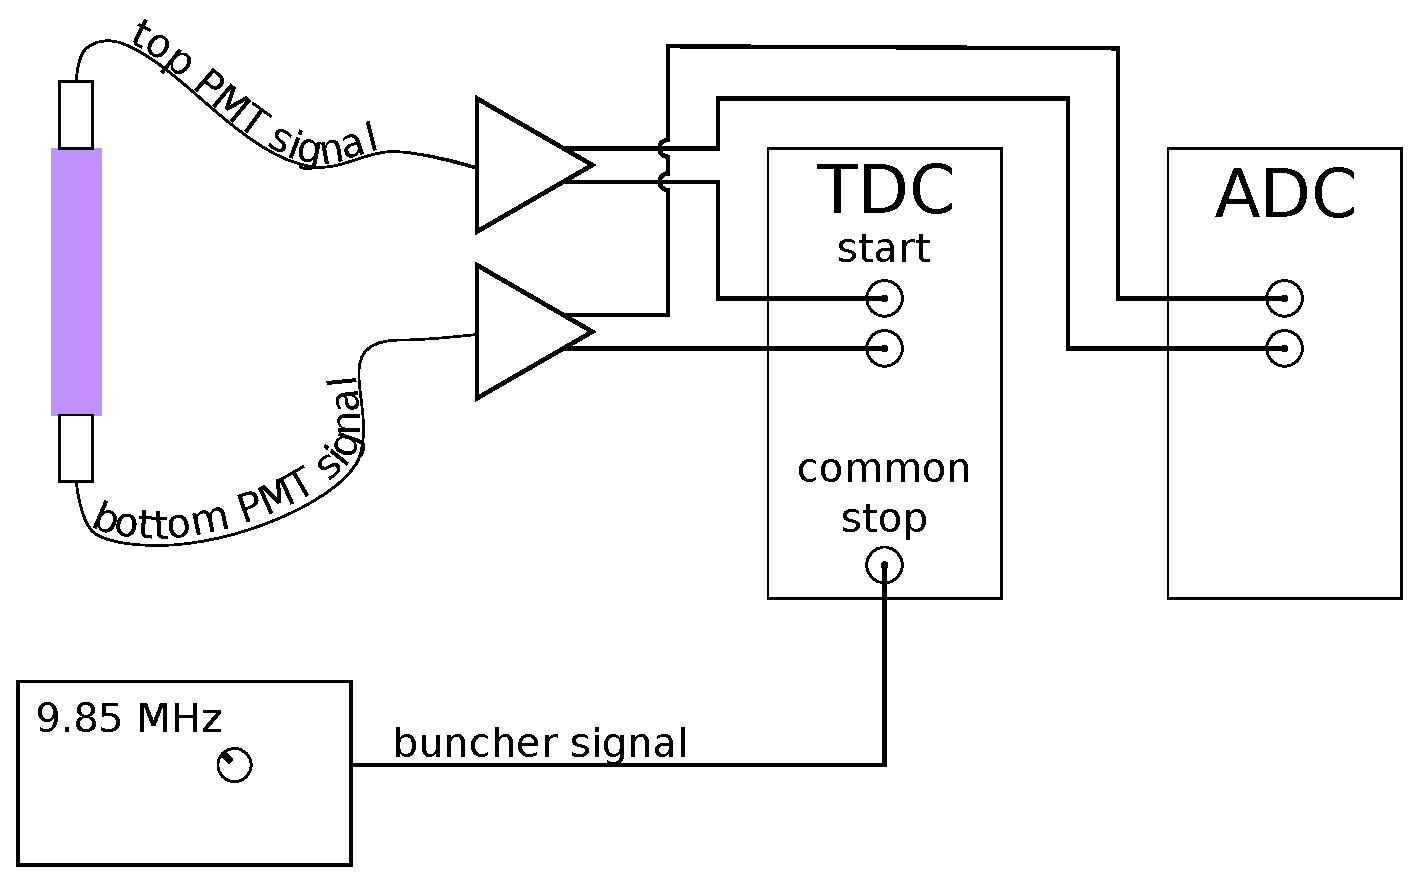
\includegraphics[width=1.0\textwidth]{figures/basic_electronics.eps}
\label{fig:simpleElectronics}
\caption{A simplified diagram of the neutron detector electronics showing the acquisition of timing and energy information from the detectors.}
\end{figure}

The fundamental components of the DAQ are the TDC, the QDC, and the event trigger that causes the DAQ to read each module.  For just one neutron detector, triggering any time either the top or bottom PMT fired would waste the DAQ with recording many noise events.  A real event should create signals in both the top and bottom PMT's, and requiring a coincidence between the two results in a reasonable trigger.  One way to define an event trigger for the entire neutron wall, then, would be to trigger any time a coincidence between associated top and bottom PMT's occurs.  But constructing this trigger with NIM logic units requires many separate logic gates and is unnecessarily complicated.  

One solution is to use the built-in OR of the CFD.  Each CFD is an eight-fold unit that provides an OR output.  Instead of requiring a top and bottom signal in the same bar, each CFD unit processes a section of only top or only bottom bar signals and the condition is loosened to requiring a signal in a top PMT and a bottom PMT in the same eight-bar group as shown in \ref{fig:eventTrig}.  The presence of some top signal AND some bottom signal triggers the event signal.  Such an event only requires that both a top and a bottom signal coincided but does not require that these signals belonged to the same bar.  Such an event trigger includes all events of interest, where the top and bottom signal belong to one bar, but also includes spurious events where no bar has signal in both its top and bottom PMT.  With a dead time of less than 30\%, this event condition does not hinder data collection, and simple software cuts eliminate spurious events.

% figure: event trigger
\begin{figure}[htp]
\centering
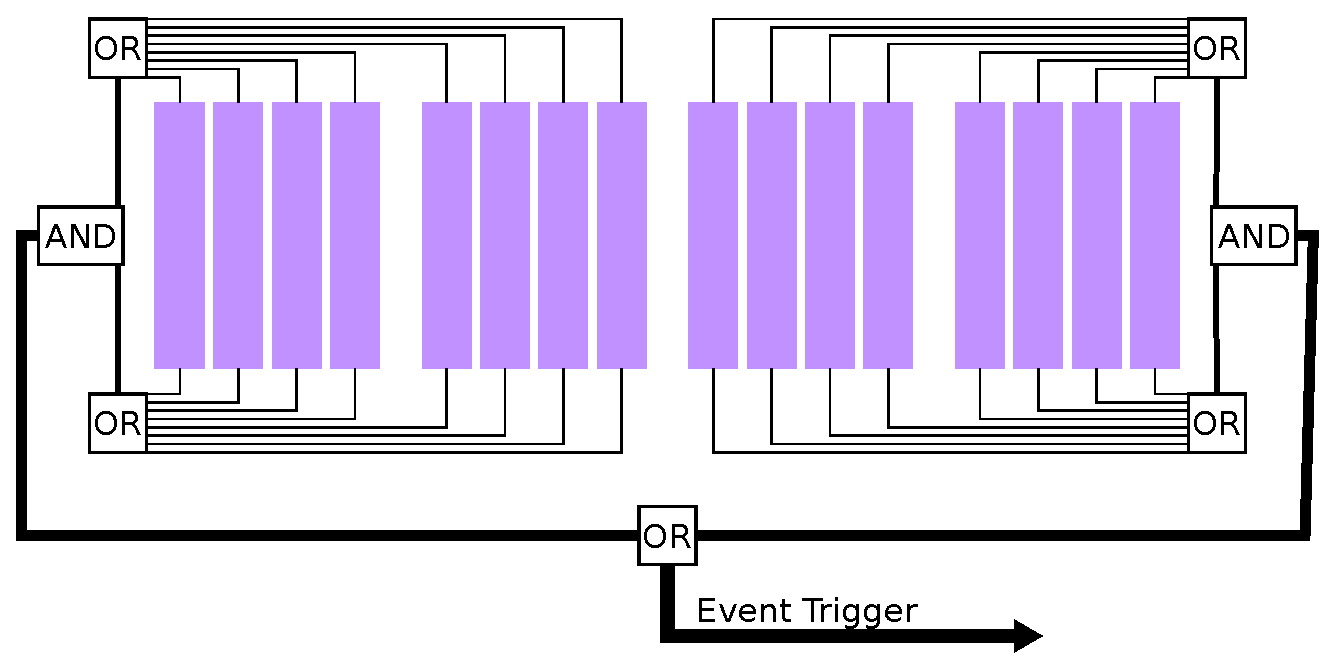
\includegraphics[width=1.0\textwidth]{figures/event_trigger.eps}
\label{fig:eventTrig}
\caption{The event trigger for the DAQ requires a coincidence between a top PMT and a bottom PMT from the same group of eight detectors.}
\end{figure}

% discuss energy, time info from near-target detectors
% and then scalers?
The time information, energy information, and a signal to indicate that this information should be read from the modules and recorded, form the core of the DAQ.  There are other quantities, however, the DAQ must record.  One of these is the dead time; the DAQ cannot collect new events while it is processing an event, and the live time is the appropriate time to use in cross-section calculation.  The DAQ itself provides two signals that allow us to measure the live time: a 100 Hz signal and a NIM logic pulse that is low when the DAQ is busy.  Vetoing the timing signal with this busy signal and recording both the un-vetoed 100 Hz signal and the busy-vetoed signal gives the ratio of live time to dead time.  The schematic is shown in figure ??.

The DAQ must also record information from the detectors near the target.  The particles of interest for the Si detector are scattered \He{3} beam, and because they are charged and deposit all their energy in the Si detector, the energy is a useful way to identify \He{3} and should be recorded.  The BaF2 detector sits outside the target chamber and monitors primarily beam-induced $\gamma$ radiation.  The timing, not energy, information of this detector is recorded by the DAQ.  Finally, because these detectors have high detection efficiency and are placed close to the target, their event rate is much higher than that of the neutron detectors.  While these detectors are essential to determining the relative particle flux through the target, the dead time they cause the DAQ should not prohibit events from the neutron detector itself from being recorded.  Running the signals from the Si and BaF2 through a pre-scaler before adding it to the event trigger limits the dead time contribution of these detectors to less than 20\%.
% figure: Si, Q.live, NaI accumulation
% figure: full electronics

A test of this electronics setup using a \Mg{26} target verified the expected DAQ operation.  This test is discussed in the next chapter. 

% % uncomment the following lines,
% if using chapter-wise bibliography
%
% \bibliographystyle{ndnatbib}
% \bibliography{example}
